\documentclass[11pt]{article}

\usepackage{authblk}
\usepackage{setspace} 
\usepackage{lineno} 
\usepackage[a4paper, margin=2cm]{geometry} 
\usepackage[parfill]{parskip}
\usepackage{graphicx} 
\usepackage[section]{placeins} 

% Harvard-style referencing
\usepackage[comma]{natbib}
\bibliographystyle{unsrt}
\setcitestyle{authoryear,open={(},close={)}}

% line numbering
\doublespacing

\title{\textbf{Bioinformatics for large-scale tumour sequence analysis}}
\author[]{Hongye Wang}
\affil[]{Imperial College London}
\date{10/12/2019}


\begin{document}
  \maketitle

\section*{}
\begin{center}
	\textbf{Supervisor:} Fumagalli Matteo, Department of Life Sciences (Silwood Park), Imperial College London
\end{center}


\newpage

\section*{Objectives}
To identify and characterise CNV (copy number variation) in tumor cells.

\section*{Introduction}
\begin{linenumbers}
Ploidy is the number of complete sets of chromosomes in a cell \cite{malhotra2015ploidy}. Individual organisms can be described according to the number of sets of chromosomes present (the “ploidy level”), like monoploid (1 set), diploid (2 sets), and cells which have three or more chromosome set are often described as polyploid. Humans are diploid organisms, carrying two complete sets of chromosomes in their somatic cells \cite{margarido2015conpade}. However, in some tumor cells, the ploidy usually increased because of the copy number variation. Therefore, we want to estimate the ploidy of tumor cells based on next generation sequencing (NGS) data and compare with the normal somatic cells.

Inferring ploidy levels is one of the most important jobs of our research. However, the current approaches can not meet our need because most of them are based on the frequency and depth of genome, they do not account for genotype uncertainty as well, that make them unreliable on low- and mid- depth sequencing data \cite{margarido2015conpade}. Instead, we choose HMMploidy as the main tool. Due to the combination of sequencing depth and genotype likelihoods, the effectiveness of HMMploidy is boosted. The great power has been shown at very low coverage in both simulated and real data.

The NGS data which I will use to analyse is collected from the patients affected by sarcoma. 

\end{linenumbers}

\title{\textbf{keywords: NGS data, Ploidy, Tumour gene sequence, CNV, HMM} 

\section*{Methods}
\begin{linenumbers}
The main method is HMMploidy. The idea is to apply this method and related software to the tumor patients’ data. The open source software is available at https://github.com/SamueleSoraggi/HMMploidy. It accepts input files in mpileup format. The framework consists of a python and R scripts (including compiled Rcpp code) \cite{bishop2006pattern}. Each script can be run with a single-line command from any UNIX shell.

\end{linenumbers}


\section*{Budget}
\begin{linenumbers}
The budget allocated towards this Master project is 500 pounds. Currently there are no expenses, however future expenses may be towards visiting and learning from interrelated research institution, attending conference and lab equipment. 
\end{linenumbers}

\section*{Schedule}
\begin{figure}[!ht]
	\centering
	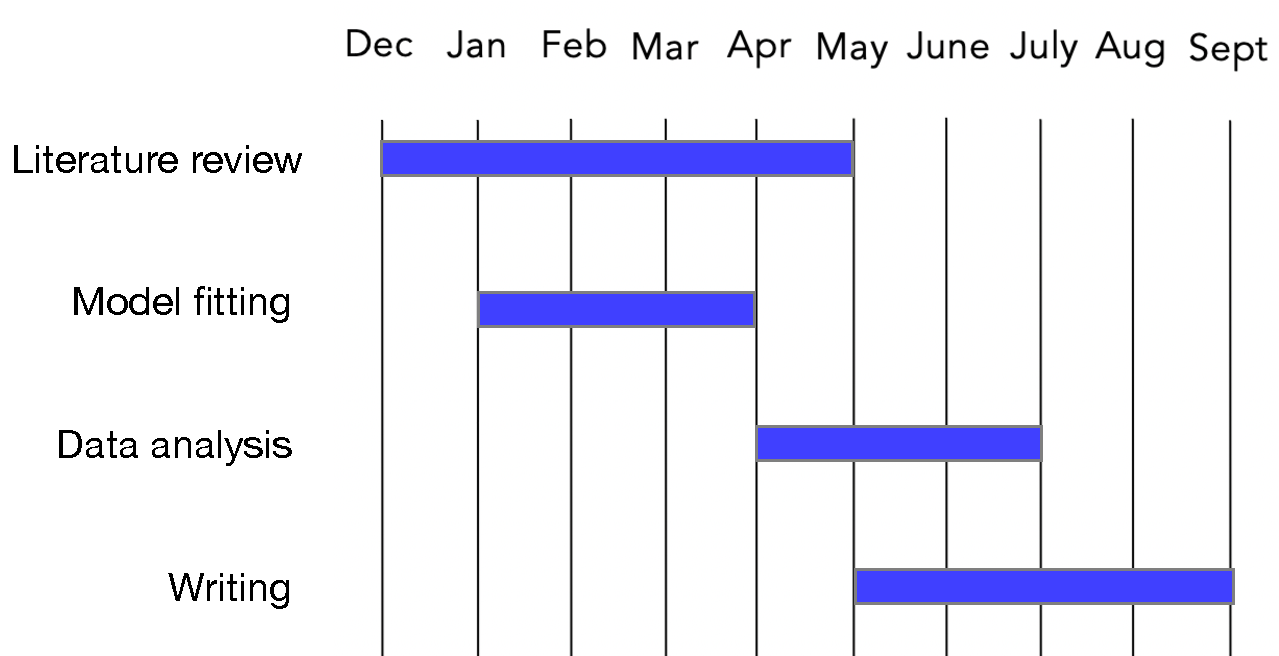
\includegraphics[scale=0.5]{./time_table.pdf} 
\end{figure}

\newpage
\thispagestyle{empty}
\section*{Supervisor Statement}
I have seen and approved the proposal and the budget.
\\
\\Supervisor: Fumagalli Matteo \\
\\
Signature: Fumagalli Matteo \\
\\
Date: 10/12/19

\bibliographystyle{plainnat}
\bibliography{proposal}

\end{document}